

%% AP Physics MC Questions Archive
%%----------------------------------------


%% Two Dimensional Collisions
%%----------------------------------------
\element{ap}{
\begin{question}{2d-collision-q01}
    Object $A$ with mass $m$ is traveling with velocity $v$ in the $x$-direction.
    Object $B$ also has mass $m$ and is traveling with velocity $v$ in the $y$-direction.
    The objects collide elastically and object $A$ rebounds with velocity $v$ in the $y$-direction.
    What is the $y$-component of the velocity of $B$ after the collision?
    \begin{multicols}{3}
    \begin{choices}
      \correctchoice{zero}
        \wrongchoice{$\dfrac{1}{2} v$}
        \wrongchoice{$v$}
        \wrongchoice{$\sqrt{2}v$}
        \wrongchoice{$2v$}
    \end{choices}
    \end{multicols}
\end{question}
}

\element{ap}{
\begin{question}{2d-collision-q02}
    Two objects of mass $m$ and $2m$ are moving horizontally parallel to the $x$-axis.
    The mass $2m$ overtakes and collides elastically with mass $m$.
    If the $y$-component of the velocity of the mass $m$ is \SI{4}{\meter\per\second} upward immediately after their collision, what is the $y$-component of the velocity of the mass $2m$ immediately after the collision?
    \begin{multicols}{2}
    \begin{choices}
        \wrongchoice{\SI{8}{\meter\per\second} downward}
        \wrongchoice{\SI{4}{\meter\per\second} downward}
      \correctchoice{\SI{2}{\meter\per\second} downward}
        \wrongchoice{\SI{4}{\meter\per\second} upward}
        \wrongchoice{\SI{8}{\meter\per\second} upward}
    \end{choices}
    \end{multicols}
\end{question}
}

\element{ap}{
\begin{question}{2d-collision-q03}
    Two balls, one of mass $m$,
        the other of mass $2m$,
        move parallel to the x-axis and collide elastically.
    If the $y$-component of the velocity of the mass $2m$ immediately after the collision is $v$,
        then the magnitude of the $y$-component of the velocity of the mass $m$ immediately after the collision is:
    \begin{multicols}{3}
    \begin{choices}
        \wrongchoice{$\dfrac{v}{3}$}
        \wrongchoice{$\dfrac{v}{2}$}
        \wrongchoice{$v$}
      \correctchoice{$2v$}
        \wrongchoice{$3v$}
    \end{choices}
    \end{multicols}
\end{question}
}

\element{ap}{
\begin{question}{2d-collision-q04}
    A cat of mass $m_c$ is sliding across a frictionless surface in the positive $x$-direction with a velocity of magnitude $v_0$ when it collides with a dog of mass $m_d$ at rest.
    \begin{center}
    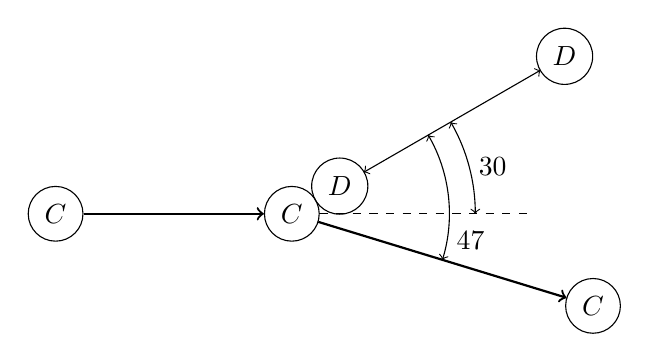
\begin{tikzpicture}
        %% Cat
        \node[circle,draw,anchor=center,minimum size=1em] (C1) at (-3,0) {$C$};
        \node[circle,draw,anchor=center,minimum size=1em] (C2) at (0,0) {$C$};
        \node[circle,draw,anchor=center,minimum size=1em] (C3) at (-17:4) {$C$};
        \draw[thick,->] (C1.east) -- (C2.west);
        \draw[thick,->] (-17:1em) -- (-17:4cm-1em);
        %% Dog
        \node[circle,draw,minimum size=1em] (D1) at (30:2em) {$D$};
        \node[circle,draw,minimum size=1em] (D2) at (30:4cm) {$D$};
        \draw[<->] (30:3em) -- (30:4cm-1em);
        %% angles
        \draw[dashed] (1em,0) -- (3,0);
        \draw[<->] (30:2.33cm) arc(30:0:2.33cm) node[pos=0.5,anchor=west] {\ang{30}};
        \draw[<->] (30:2cm) arc(30:-17:2cm) node[pos=0.85,anchor=west] {\ang{47}};
    \end{tikzpicture}
    \end{center}
    The dog now travels at an angle \ang{30} with respect to the cat's initial path at a velocity of magnitude $v_1$.
    The cat travels at an angle of negative \ang{47} with respect to the dog's path of motion with a velocity of magnitude $v_2$.
    Which of the following is true?
    \begin{choices}
      \correctchoice{$m_d v_1\sin\ang{30} = m_c v_2\sin\ang{17}$}
        \wrongchoice{$m_d v_1\sin\ang{30} = m_c v_2\sin\ang{47}$}
        \wrongchoice{$m_d v_1\cos\ang{30} = m_c v_2\cos\ang{17}$}
        \wrongchoice{$m_d v_1\cos\ang{30} = m_c v_2\cos\ang{47}$}
        \wrongchoice{$m_d v_1\sin\ang{30} + m_c v_2\sin\ang{17} = m_c v_0$}
    \end{choices}
\end{question}
}

\element{ap}{
\begin{question}{2d-collision-q05}
    A \SI{1.0}{\kilo\gram} mass traveling \SI{3.0}{\meter\per\second} north and a \SI{2.0}{\kilo\gram} mass traveling \SI{2.0}{\meter\per\second} east collide and stick together.
    After the collision,
        their speed is most nearly:
    \begin{multicols}{3}
    \begin{choices}
        \wrongchoice{\SI{1.0}{\meter\per\second}}
      \correctchoice{\SI{1.7}{\meter\per\second}}
        \wrongchoice{\SI{2.5}{\meter\per\second}}
        \wrongchoice{\SI{3.2}{\meter\per\second}}
        \wrongchoice{\SI{5.0}{\meter\per\second}}
    \end{choices}
    \end{multicols}
\end{question}
}

\element{ap}{
\begin{question}{2d-collision-q06}
    %% Base your answers to questions 6 and 7 on the following situation.
    An object with a mass of 6.0 kilograms and a velocity of \SI{4.0}{\meter\per\second} in the $x$-direction collides with an object of mass \SI{3.0}{\kilo\gram} and a velocity of \SI{8.0}{\meter\per\second} in the $y$-direction and they stick together.
    %% Start question
    After the collision,
        the angle the objects' trajectory makes with the $x$-axis is most nearly:
    \begin{multicols}{3}
    \begin{choices}
        \wrongchoice{\ang{0}}
        \wrongchoice{\ang{30}}
      \correctchoice{\ang{45}}
        \wrongchoice{\ang{60}}
        \wrongchoice{\ang{90}}
    \end{choices}
    \end{multicols}
\end{question}
}

\element{ap}{
\begin{question}{2d-collision-q07}
    %% Base your answers to questions 6 and 7 on the following situation.
    An object with a mass of 6.0 kilograms and a velocity of \SI{4.0}{\meter\per\second} in the $x$-direction collides with an object of mass \SI{3.0}{\kilo\gram} and a velocity of \SI{8.0}{\meter\per\second} in the $y$-direction and they stick together.
    %% Start question
    After the collision the velocity of the objects is most nearly:
    \begin{multicols}{3}
    \begin{choices}
        \wrongchoice{\SI{2.3}{\meter\per\second}}
      \correctchoice{\SI{3.7}{\meter\per\second}}
        \wrongchoice{\SI{4.5}{\meter\per\second}}
        \wrongchoice{\SI{6.9}{\meter\per\second}}
        \wrongchoice{\SI{7.0}{\meter\per\second}}
    \end{choices}
    \end{multicols}
\end{question}
}

\element{ap}{
\begin{question}{2d-collision-q08}
    An object at rest splits into 3 particles, each with mass $m$,
        traveling with velocity $v$.
    The angle between the velocity vectors of any two of these particles is:
    \begin{multicols}{3}
    \begin{choices}
        \wrongchoice{\ang{30}}
        \wrongchoice{\ang{60}}
        \wrongchoice{\ang{90}}
      \correctchoice{\ang{120}}
        \wrongchoice{\ang{150}}
    \end{choices}
    \end{multicols}
\end{question}
}


\endinput


